\loesung{	
	\begin{enumerate}[a)]
		\item Permutation Feature Importance compares the performance of the model on the original data with the performance on perturbed data, where the dependence of the variable of interest (let's call it $x_j$) with the target $Y$ variable is broken.
		
		In order to break the dependence of $x_j$ with $y$, $x_j$ is replaced with a permuted version $\tilde{x}_j$ which is independent of the target.
		
		However, by permuting the variable we do not only break the dependence with $y$, but also with all other covariates. As such, we may create unrealistic observations.
		
		For example, time of the year may be dependent with the highest temperature on a day. If we resample the variable time of the year independently of the temperature high, we may create observations where time of the year is winter and temperature high is 40 degrees celsius.
		\item If a feature anyway independent of its covarites ($x_j\perp x_{-j}$, then PFI does not extrapolate to unseen regions.
		
		Intuitively, the reason is that no dependence with the covariates is broken, since there were not dependencies between $x_j$ and the remaining variables $x_{-j}$ to begin with..
		
		\item Pseudocode reading in data, estimating a regression model and calculating the MSE
		\begin{algorithm}[H]
			\caption{getting started}
			\begin{algorithmic}[1]
				\State \texttt{df} $\gets$ read in dataset \texttt{extrapolation.csv}
				\State \texttt{X, y} $\gets$ features, target
				\State \texttt{X\_train, X\_test} $\gets$ training data, test data
				\State \texttt{model} $\gets$ linear regression model on \texttt{X\_train}
				\State \textbf{return} MSE of \texttt{model} predictions
			\end{algorithmic}
		\end{algorithm}
		
		\item First, we implement PFI. Here we implement the methods generically, such that the perturbation mechanism can easily be replaced. Therefore, we make use of \texttt{f(*args,**kwargs)} and \texttt{f(...)} in Python and R, respectively.
		
		Pseudocode of \texttt{pfi\_fname()}
		
		\begin{algorithm}[H]
			\caption{\texttt{pfi\_fname()}}
			\begin{algorithmic}[1]
				\Require \texttt{fname}: feature of interest name
				\Require \texttt{predict}: prediciton function
				\Require \texttt{score}: performance metric
				\Require \texttt{X\_test}: data for the evaluation
				\Require \texttt{y\_test}: respective labels
				\Require \texttt{...}: further arguments (which are ignored)
				\State \texttt{X\_test\_perturbed} $\gets$ copy \texttt{X\_test} and randomly permute column containing feature \texttt{fname}
				\State \texttt{performance} $\gets$ \texttt{score(y\_test, predict(X\_test\_perturbed)) - score(y\_test, predict(X\_test))}
				\State \textbf{return} \texttt{performance}
			\end{algorithmic}
		\end{algorithm}
		
		Pseudocode of \texttt{fi\_naive()}
		
		\begin{algorithm}[H]
			\caption{\texttt{fi\_naive()}}
			\begin{algorithmic}[1]
				\Require \texttt{perf\_pert}: function that returns performance for some perturbation.
				\Require \texttt{predict}: prediciton function
				\Require \texttt{score}: performance metric
				\Require \texttt{X\_test}: data for the evaluation
				\Require \texttt{y\_test}: respective labels
				\Require \texttt{...}: further arguments (which are ignored)
				\For{\texttt{fname} in columns of \texttt{X\_test}}
				\State \texttt{imp} $\gets$ \texttt{fi\_fname(fname, predict, score, X\_test, y\_test, ...)}
				\State \texttt{results} $\gets$ extend by \texttt{imp}
				\EndFor
				\State \textbf{return} \texttt{results}
			\end{algorithmic}
		\end{algorithm}
		
		Pseudocode of \texttt{n\_times()}
		
		\begin{algorithm}[H]
			\caption{\texttt{n\_times()}}
			\begin{algorithmic}[1]
				\Require \texttt{n}: number of repetitions
				\Require \texttt{method}: feature importance method.
				\Require \texttt{args}: all further arguments that are required for the method
				\Require \texttt{return\_raw}: Whether only the aggregation (mean, stdd) or also the raw results are returned
				\For{\texttt{i} in \texttt{n}}
				\State \texttt{tmp} $\gets$ \texttt{method(args)}
				\State \texttt{results} $\gets$ extend by \texttt{tmp}
				\EndFor
				\State \texttt{mean\_fi} $\gets$ mean of \texttt{results}
				\State \texttt{std\_fi} $\gets$ stdd of \texttt{results}
				\If{\texttt{return\_raw} equals \texttt{True}} \textbf{return} \texttt{mean\_fi, std\_fi, raw\_results}
				\ElsIf{\texttt{return\_raw} equals \texttt{False}} \textbf{return} \texttt{mean\_fi, std\_fi}
				\EndIf
			\end{algorithmic}
		\end{algorithm}
		
		Now we apply the method to our model and dataset.
		\begin{algorithm}[H]
			\caption{application}
			\begin{algorithmic}[1]
				\State \texttt{nr\_runs} $\gets$ 10
				\State \texttt{fis\_mean, fis\_std} $\gets$ \texttt{n\_times(nr\_runs, fi\_naive, pfi\_fname, model} prediction function, \texttt{mean\_squared\_error, X\_test, y\_test, return\_raw=False)}
				\State \texttt{plot} bar chart
			\end{algorithmic}
		\end{algorithm}
		
		\item $X_3$ is the most important feature, with $X_1$ and $X_2$ sharing the second place. PFI considers $X_4$ to be irrelevant.
		
		According to the PFI interpretation rules, without further assumptions about the data, we know that
		\begin{itemize}
			\item $X_1$, $X_2$, $X_3$ are used by the model for it's prediction
			\item $X_1$, $X_2$, $X_3$ are dependent with $Y$ and/or dependent with the covariates
			\item $X_4$ may be independent of $Y$ and covariates and/or not used by the model. We only know that it is not both dependent and used by the model.
		\end{itemize}
		Bonus: If we would additionally analyze the data we find out that $X_1, X_2$ are dependent but $X_3$ is independent of all covariates.
		
		As such, we could further conclude that $X_3$ is dependent with $Y$ (but do not know for $X_1$, $X_2$ without looking into the data).
		
		\item Correlation matrix: 
		\begin{table}[H]
			\centering
			\begin{tabular}{l|lllll}
				\hline
				& $x_1$ & $x_2$ & $x_3$ & $x_4$ & $y$ \\
				\hline
				$x_1$ &  1.0*** &  1.0*** &  0.03 & -0.05 &  0.02 \\
				$x_2$ &  1.0*** &  1.0*** &  0.03 & -0.05 &  0.02 \\
				$x_3$ &  0.03 &  0.03 &  1.0*** & -0.0 &  1.0*** \\
				$x_4$ & -0.05 & -0.05 & -0.0 &  1.0*** &  0.0 \\
				$y$ &  0.02 &  0.02 &  1.0*** &  0.0 &  1.0*** \\
				\hline
			\end{tabular}
		\end{table}
		Our interpretation was correct.
		
		\item If we know the dependence structure of the covariates we can infer whether or not the PFI value is nonzero due to a dependence with the covariates or not. In our example we now know that $x_3$ is independent of its covariates, so we hypothesize that $x_3$ is actually dependent with $y$ (and would perform importance tests as a consequence). Since $x_1, x_2$ are dependent, for those variables we cannot infer anything about the dependence with $y$ with the covariates dependence structure and PFI alone.
		
		\item We use the \texttt{extrapolation.csv} dataset. We create a pairplot showing the pairwise scatterplot of the original feature as well as the corresponding perturbed variable with all remaining feature variables (and potentially $y$).
		\begin{center}
			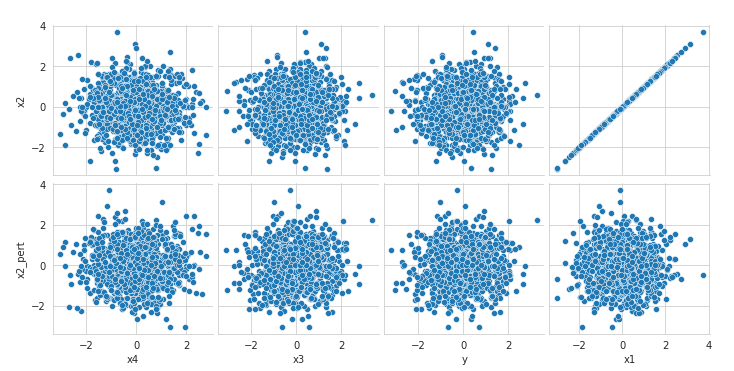
\includegraphics[width = .7\textwidth]{"figure/pairplot_comparison.png"}
		\end{center}
		We can see that the strong correlation of $x_2$ with $x_1$ (top row) is broken after permutation (bottom row). All other pairwise (in)dependencies are unchanged. Note: We only assess pairwise, unconditional dependencies. Without assumptions about the data, we cannot know whether further conditional depencies with the remaining covariates were broken.
		
	\end{enumerate}
}
